\section{Modelling Previous Design}\label{sec:old-design-method}
Because microgravity is incredibly costly to achieve experimentally, a numerical investigation of the previous design was conducted using ANSYS Fluent. The simulation was run twice, once with gravity and once without, to compare the distribution of powder within the tank and the resulting mass flow rate. 

Initially, an axisymmetric simulation using square cells of 0.4mm was attempted. This configuration was chosen because it could run as quickly as a 2D simulation, due to the reduced number of cells, while still capturing the 3D physics of the real system. It was assumed that the fine mesh allowed for strong, non-physical, flow gradients to be resolved as the simulation was numerically unstable and repeatedly crashed. To address this, a new 2D simulation with a coarser mesh of 1mm square cells was performed, shown in \autoref{fig:old-design-sim}.
\begin{figure}[htbp]
    \centering

    \begin{minipage}{0.25\textwidth}
        \centering
        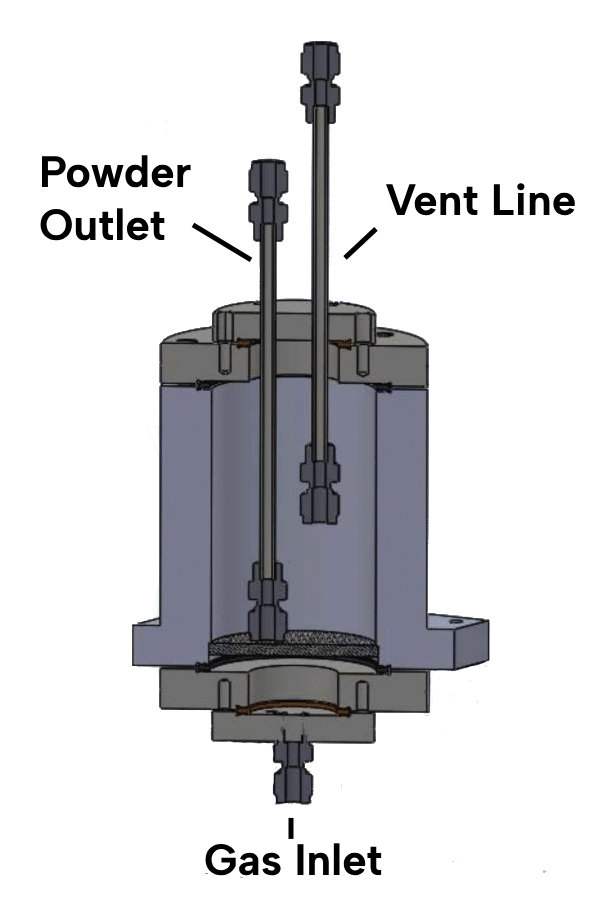
\includegraphics[width=\textwidth]{../report_assets/COSMOS_DIAGRAM_2_3.png}
        \caption*{(a) Previous Design}
    \end{minipage}
    \hfill
    \begin{minipage}{0.25\textwidth}
        \centering
        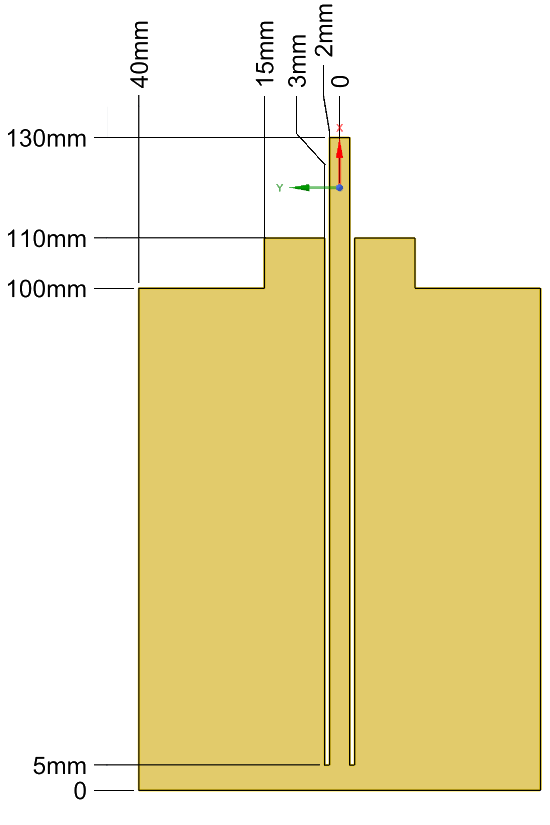
\includegraphics[width=\textwidth]{../report_assets/geom_old.png}
        \caption*{(b) Simplified Geometry}\label{fig:idkyet9}
    \end{minipage}
    \hfill
    \begin{minipage}{0.25\textwidth}
        \centering
        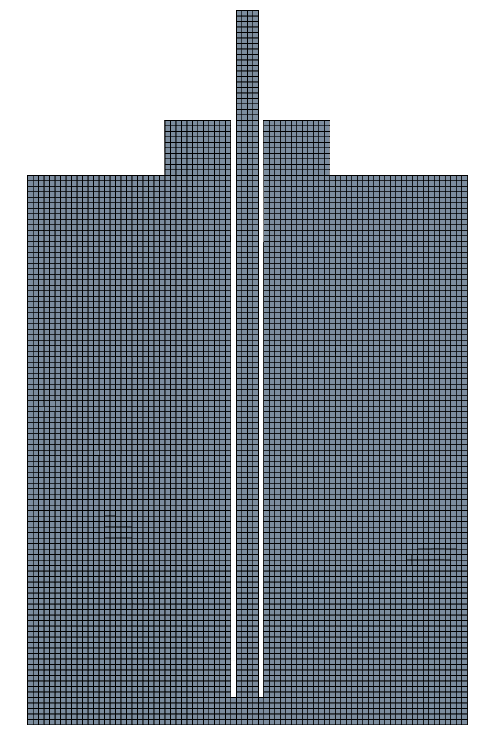
\includegraphics[width=\textwidth]{../report_assets/mesh_old.png}
        \caption*{(c) Mesh Used for Sim}\label{fig:idkyet10}
    \end{minipage}
    
\end{figure}\label{fig:old-design-sim}
While the 2D nature of the simulation means the quantities such as mass flow rate and inlet conditions can not be matched exactly to the real system, the key flow characteristics of interest are still expected to persist. This is because particle position within the tank and the onset of fluidisation are not strongly dependent on three-dimensional effects.

A simplified geometry, seen in \autoref{fig:old-design-sim} (b), was used to reduce computational time while preserving the essential geometric features. It is important to note that the vent line pipe was omitted and the outlet pipe was moved to the center; neither of these modifications are expected to affect the behaviour under investigation. 

The bottom of the tank held a wire mesh on which the powder rested, representing the lower geometric boundary. In the simulation, this mesh acted as a velocity inlet, with gas entering the system at a velocity of 0.1m/s. 

To simulate the two gas and powder phases, an Eulerian-Eulerian model was employed along with the Gidaspow drag model, which has been shown to best represent fluidised beds~\cite{C6RA28615A}. The powder was modelled as TI6AL4V, consistent with the material used during COSMOS.\@ Titanium alloy powder used in selective layer sintering (SLS) have a particle size distribution between $15\,\mu\mathrm{m}$ and $53\,\mu\mathrm{m}$ and a density ranging from $2.04\ \mathrm{g/cm^3}$ to $2.34\ \mathrm{g/cm^3}$~\cite{ma17040952}, which is assumed to be similar to the powder used in CSAM.\@ Hence a representative particle size of $40\,\mu\mathrm{m}$ and a density of $2200\ \mathrm{kg/m^3}$ were used. 

The gas was modelled as nitrogen at standard operating conditions, consistent with its use in COSMOS.\@

\section{Choosing A New Feed System Architecture}\label{sec:system_architecture}
As discussed in \autoref{sec:prev-design-analysis}, the results of the analysis into the previous design supported the hypothesised issues. Consequently, a new design was deemed necessary, and a review of current powder feed technologies was conducted to better understand the strengths and limitations of prior systems. Although a thorough review of analogous systems was undertaken, it remains possible that some key papers were overlooked. The only research found on powder-based AM experiments conducted in microgravity originate from the Fraunhofer Institute; yet, this report offers limited detail on the powder-feed mechanism employed~\cite{OVERMEYER2025}. 

Accordingly, five common terrestrial powder-dispensing methods, shown in \autoref{fig:powder-dispensing-methods}, were examined, comparing both their suitability for use in the space environment without modifications and the complexity of implementing any necessary adaptations. 
\begin{figure}[htbp]
    \centering

    % First row: 3 images
    \begin{minipage}{0.3\textwidth}
        \centering
        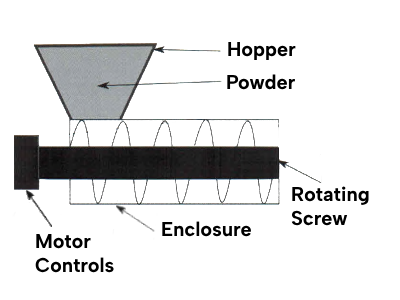
\includegraphics[width=\textwidth]{../report_assets/screw_feed_polished.png}
        \caption*{(a) Screw Fed Design~\cite{Bitragunta2015}}
    \end{minipage}
    \hfill
    \begin{minipage}{0.3\textwidth}
        \centering
        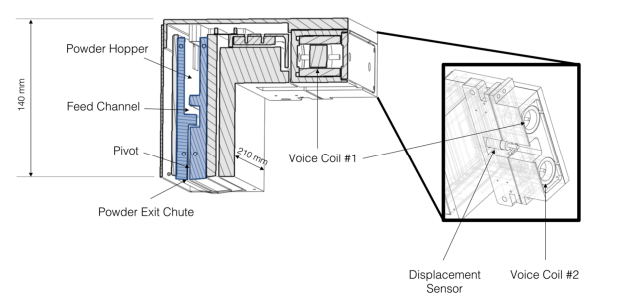
\includegraphics[width=\textwidth]{../report_assets/vibrational_feed.png}
        \caption*{(b) Vibration Fed Design~\cite{Sinclair2021}}
    \end{minipage}
    \hfill
    \begin{minipage}{0.3\textwidth}
        \centering
        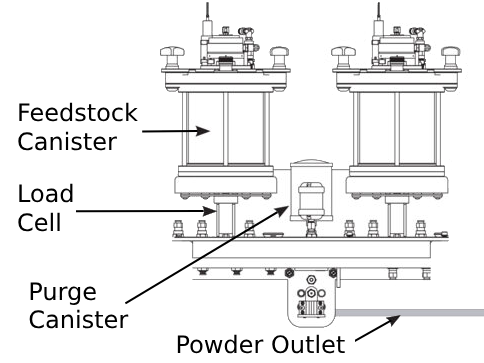
\includegraphics[width=\textwidth]{../report_assets/Liquid_oerlikon.png}
        \caption*{(c) Liquid Suspension Design~\cite{OerlikonMetcoFeeders2023}}
    \end{minipage}
    % Second row: 2 images
    \begin{minipage}{0.35\textwidth}
        \centering
        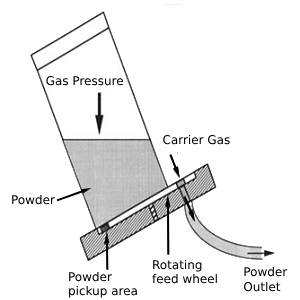
\includegraphics[width=\textwidth]{../report_assets/rotating_disk.png}
        \caption*{(d) Rotating Disk Design~\cite{Crawmer2013}}
    \end{minipage}
    \hspace{0.1\textwidth}
    \begin{minipage}{0.35\textwidth}
        \centering
        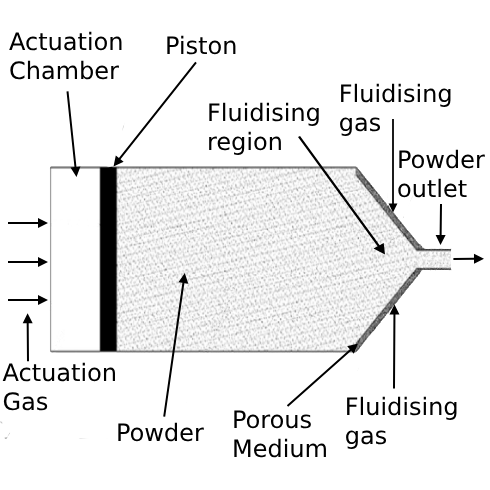
\includegraphics[width=\textwidth]{../report_assets/fluidising_powder_design.png}
        \caption*{(e) Fluidised Powder Bed Design~\cite{Li2016}}
    \end{minipage}
    
    \caption{5 Common Powder Feed System Architectures}\label{fig:powder-dispensing-methods}
\end{figure}
Only basic schematics of these methods are presented as the details of the unselected architectures are not relevant and the selected architecture is already outlined in \autoref{sec:fluidised-powder-feed-systems}. The full analysis is tabulated in \autoref{appendix:feed-architecture-analysis}. The fluidised powder bed design was selected as the most promising architecture because, like the CSAM method itself, it requires pneumatic systems, thereby mitigating this as a drawback when compared to other architectures. Furthermore, this method is assumed to be less affected by microgravity than other options, as the dominant forces acting on the particle are fluid mechanical in nautre, requiring no adjustments of the core mechanic of feeding. 

As discussed in \autoref{sec:fluidised-powder-feed-systems}, the fluidised powder bed architecture has gone through a number of design iterations since its first implementation, primarily driven by miniaturisation requirements. To align this investigation with state-of-the-art systems, the pneumatically driven, permiable piston architecture was selected. 

\section{Hopper Tank Design}
In fluidised powder feed systems, the tank serves a dual purpose. When not in operation, it acts as a storage vessel, securely holding the powder in a fluidisable state. During operations, the same tank functions as a delivery mechanism, enabling controlled powder dispensing through piston actuation and the introduction of fluidising gas. 

Based on prior experience with the CSAM system used in COSMOS, successful samples were produced with inlet pressures between 5 and 8 bar. Therefore, 8 bar was selected as the design operating pressure for the tank. It is expected that this subsystem will experience pressure lower than or equal to the rest of the system and therefore be able to facilitate tests with an inlet pressure of 8 bar. 

Although the standard safety factor for pressure vessels is 3.5 to 4~\cite{redriver2024asme}, this was not known at the time of design and was only discovered after manufacturing. In future iterations, this would be addressed by increasing wall thinkness of the tank as well as using radial bolts to secure the outlet end cap to the tube.

The end caps were manufactured from Acetal C POM Delrin due to its is low-cost, ease of machining and chemical inertness. The main tube was made from clear acrylic to allow for visual ovservations of flow behaviour. Upon evaluation, polycarbonate would have been a more suitable material, as it is significantly less prone to shattering~\cite{SADEGHIESFAHLANI2021e06856}.
\begin{figure}[htbp]
    \centering

    \begin{minipage}{0.3\textwidth}
        \centering
        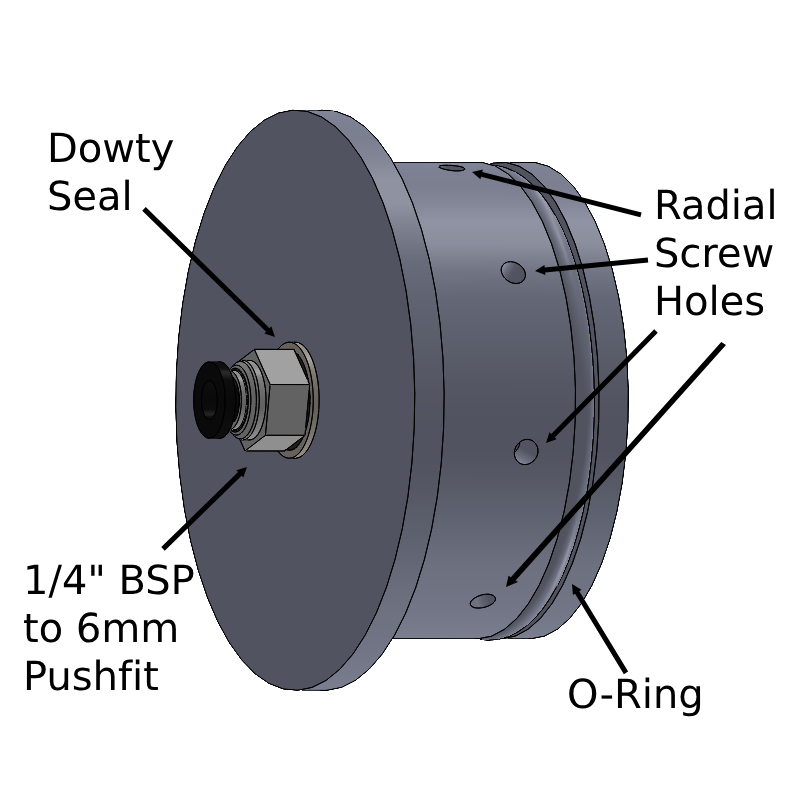
\includegraphics[width=\textwidth]{../report_assets/inlet_end_cap.png}
        \caption*{(a) Inlet End Cap}
    \end{minipage}
    \hfill
    \begin{minipage}{0.3\textwidth}
        \centering
        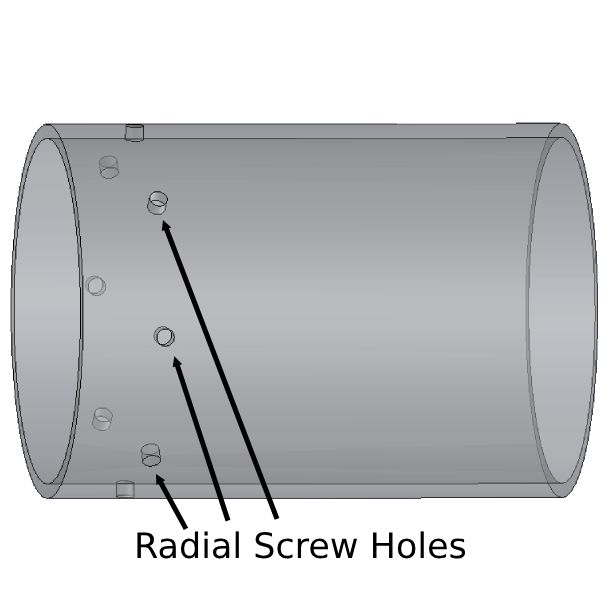
\includegraphics[width=\textwidth]{../report_assets/tube.png}
        \caption*{(b) Acrylic Tube}
    \end{minipage}
    \hfill
    \begin{minipage}{0.3\textwidth}
        \centering
        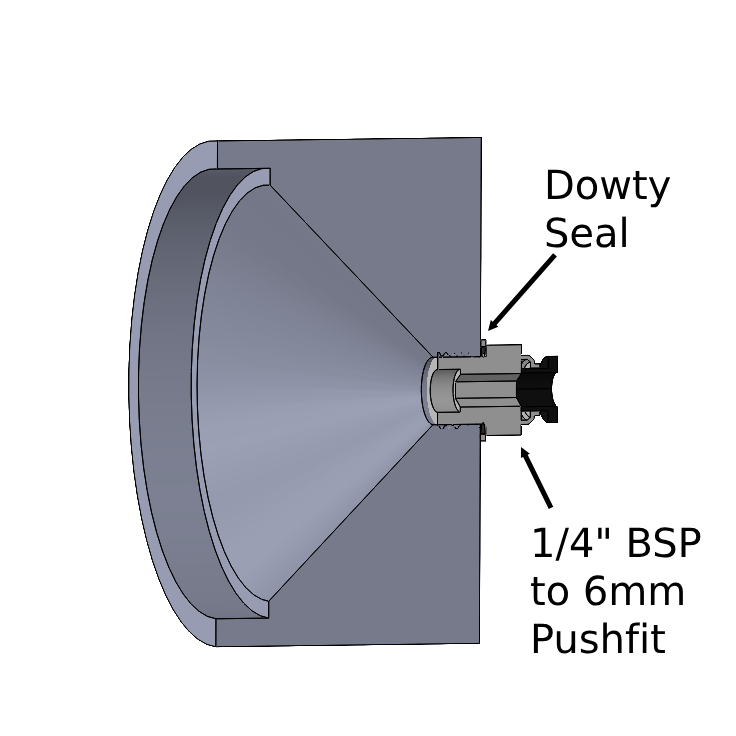
\includegraphics[width=\textwidth]{../report_assets/outlet_end_cap.png}
        \caption*{(c) Outlet End Cap Cross Section}
    \end{minipage}
    \caption{Components of the Hopper Tank}\label{fig:hopper-tank-components}
\end{figure}
As seen in \autoref{fig:hopper-tank-components}, the inlet end cap is radially screwed into the tube. This design choice was made to allow the end cap to be removed for testing different piston designs. The outlet end cap was bonded to the tube using a plastic-compatible epoxy adhesive.

\section{Hopper Tank Analysis}\label{sec:tank-fea-setup}
To validate that the design could operate up to a pressure up to 8 bar during experimentation, a combination of hand calculations and finite element analysis (FEA) using SolidWorks was performed. The failure modes analysed included stress concentrations around the bolt holes and hoop stress rupture. Fracturing at the Delrin-epoxy interface was also a concern; however, due to the lack of relevant literatures on modelling this behaviour, it was not investigated further. Bolt tear-out was not analysed, as the number and length of bolts made it an unlikely failure mode.

To assess the stress distribution around the bolt holes, a static force simulation was conducted using two different mesh resolutions, as shown in \autoref{fig:solidworks-fea}. 
\begin{figure}[htbp]
    \centering

    \begin{minipage}{0.45\textwidth}
        \centering
        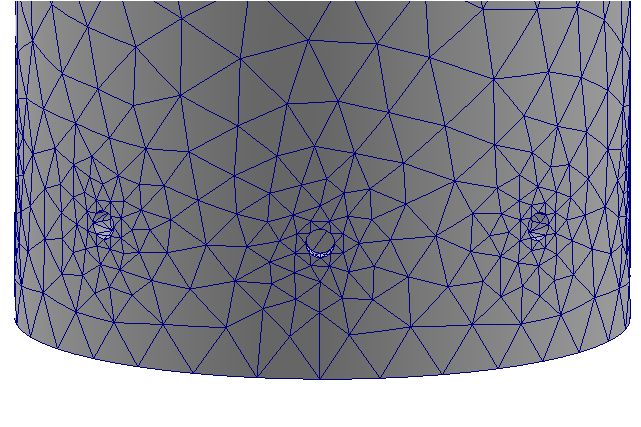
\includegraphics[width=\textwidth]{../report_assets/fine_mesh.png}
        \caption*{Mesh with Fine Setting}
    \end{minipage}
    \hfill
    \begin{minipage}{0.45\textwidth}
        \centering
        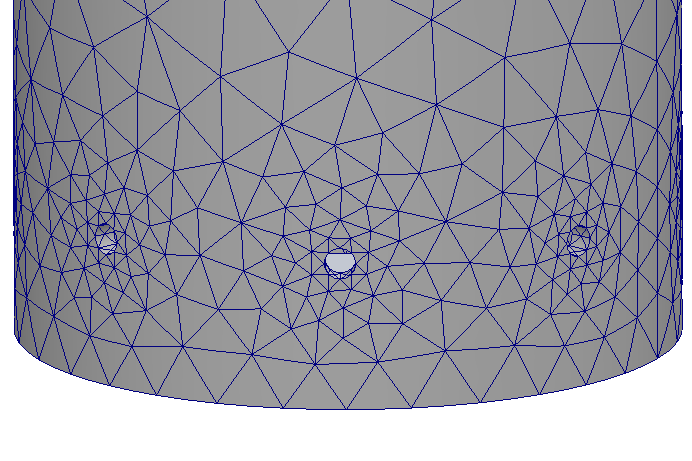
\includegraphics[width=\textwidth]{../report_assets/medium_mesh.png}
        \caption*{Mesh with More Coarse Setting}
    \end{minipage}
    \caption{Solidworks Meshes Used to Analyse Tank Design}\label{fig:solidworks-fea}
\end{figure}
The force on the bolt holes was assumed to result from the pressure acting on the end cap face due to a 7 bar pressure differential, neglecting any effect from the O-ring seal. This force was calculated using the equation:
\[
F = P \cdot A
\]
\[
F = 700,000Pa \cdot (0.037m^2 \cdot \pi) = 3,010N
\]
This force was applied to only the bottom half of each bolt hole's cross-section, representing the region where the bolt makes contact with the surface. The acrylic was modelled using SolidWorks' predefined medium-high impact acrylic, with a Young's modulus of 3 GPa and a yield stress of 45 MPa. 

These material properties were also used in hand calculations to investigate hoop stress rupture as a potential failure mode. The tank was treated as a thick-walled cylinder and hoop stress was calculated using Lamé's equation~\cite{mydatabook_lame}: 
\[
\sigma_\theta(r) = \frac{p_i r_i^2 - p_o r_o^2}{r_o^2 - r_i^2} + \frac{(p_o - p_i) r_i^2 r_o^2}{(r_o^2 - r_i^2) r^2}
\]
where the outer radius, $r_o$, was 0.04m and the inner radius, $r_i$, was 0.037m. The external pressure, $p_o$, was taken as atmospheric (approximately 1 bar) and the internal pressure, $p_i$, was modelled as 8 bar.
\section{Piston Design}\label{sec:piston}
The primary function of the piston in this design is to constrain the powder at the outlet of the device. By modelling the powder as a fluid, the force required by the piston to pack the sand against the outlet can be calculated through the hydrostatic pressure equation: 
\[
P = \rho * h * g
\]
The pressure differential across the piston generated by the fluidising gas flow must counteract both this pressure from the powder and the frictional force between the piston and the tank walls to ensure effective compaction. However, due to the non-linear nature of granular material's affect on friction, modelling this interaction in detail was deemed beyond the of the scope of the project. Additionally, manufacturing imperfections in both the tank tube and piston prevented accurate modelling of the flow field around the piston, making the expected pressure differential across it too complex to simulate reliably. Although the piston design holds significant potential for system optimisation, time constraints of the project limited further investigation.

Given these complexities, the initial piston geometry, seen in \autoref{fig:piston_geom} (a), was modelled after a previous study, which found that a gear-like geometry offered the best performance in a gas-permeable powder feed system~\cite{TANG2023118406}. 
\begin{figure}[htbp]
    \centering
    
    \begin{minipage}{0.29\textwidth}
        \centering
        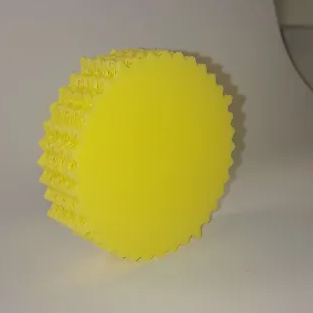
\includegraphics[width=\textwidth]{../report_assets/piston_1.png}
        \caption*{(a) First Design}\label{fig:piston_geom_1}
    \end{minipage}
    \hfill
    \begin{minipage}{0.29\textwidth}
        \centering
        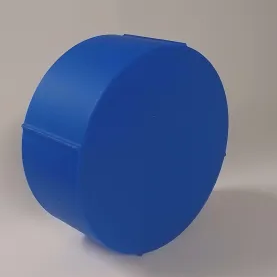
\includegraphics[width=\textwidth]{../report_assets/piston_2.png}
        \caption*{(b) Second Design}\label{fig:piston_geom_2}
    \end{minipage}
    \hfill
    \begin{minipage}{0.29\textwidth}
        \centering
        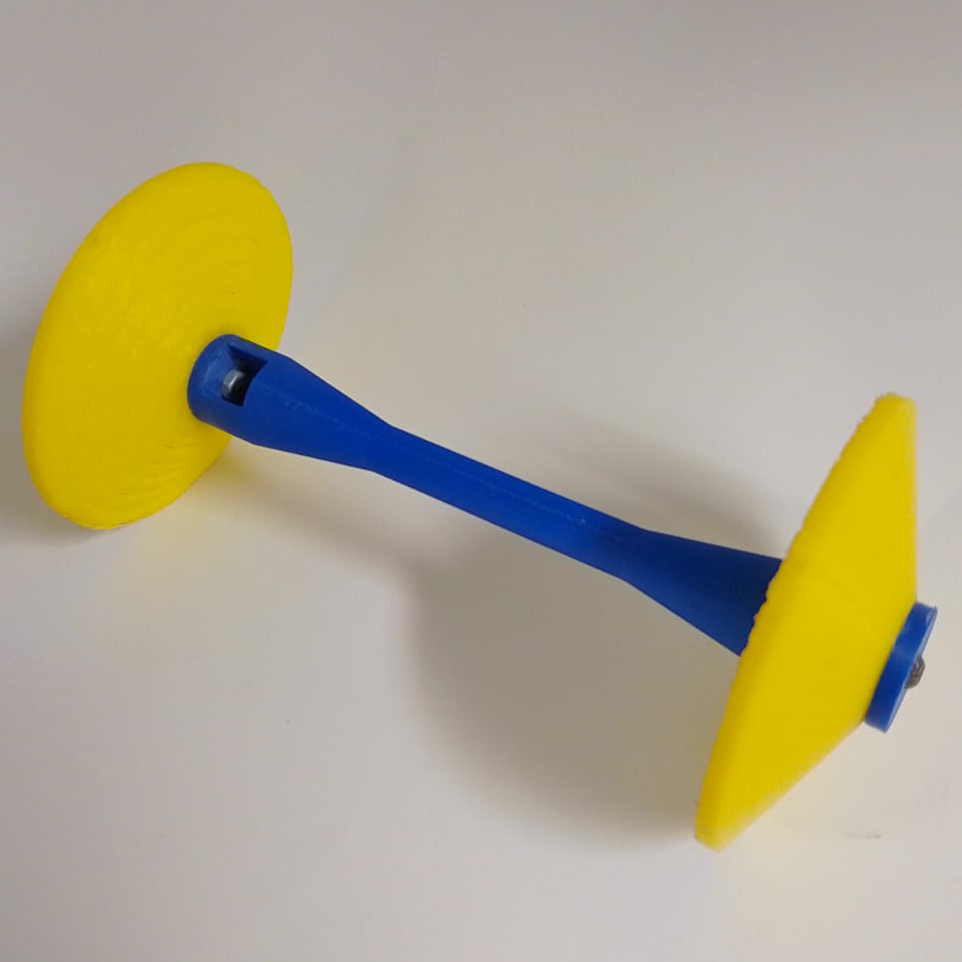
\includegraphics[width=\textwidth]{../report_assets/piston_final.png}
        \caption*{(c) Final Design}\label{fig:piston_geom_3}
    \end{minipage}
    \caption{Piston Design Iterations}\label{fig:piston_geom}
\end{figure}
The first piston was designed under the assumption that the high pressure within the tank would not equalise quickly enough with the pressure inside the printed piston, causing it to crumple or deform. To address this, the wall layers were omitted during 3D printing to allow for pressure equalisation. However preliminary testing revealed that this design did not generate sufficient pressure force to move down the tank, prompting a second iteration.

Building on this insight, the second piston was designed to constrict the flow around its perimeter as much as possible to increase the pressure differential acting on it. As discussed in \autoref{sec:first-test}, this piston was able to move under pressure but became immediately jammed by the sand, motivating the third redesign focused on preventing jamming.

The final piston consists of 2 3D-printed TPU cones, each 3mm thick, connected by a 100mm PLA rod. The flexibility of TPU provided critical resiliance against jamming, allowing individual grains to be flexed around so that the piston could continue compacting the remaining sand. In addition to the material change, increasing the piston's length helped mitigate jamming due to axis misalignment. 

The dual-plate and rod configuration not only resulted in a lighter design compared to a fully TPU piston, but also reduced the contact area, lowering the risk of frictional sticking or sand-induced jamming. Moreover, the compliant nature of TPU enabled the piston face to conform to the tank's internal surface, compensating for manufacturing imperfections such as slight variations in diameter or cylindricity. This allowed for a more effective seal, enabling higher pressure differentials and more consistent compaction of the sand at the outlet.
% why is axis-misalignment solved by making it longer

\section{Expected Behaviour}\label{sec:expected-behaviour}
To predict the behaviour of the system, parallels were drawn from research looking at fluidising powder feed systems for metal powder engines. It has been proposed that the flow behaviour within the tank can be divided into two distinct regions: a dense phase moving area preceding the cone, and a fluidising region afterwards~\cite{Tang22}. This conceptual model is interpreted in the behaviour illustrated in \autoref{fig:expected}. 
\begin{figure}[htbp]
    \centering
    
    \begin{minipage}{0.6\textwidth}
        \centering
        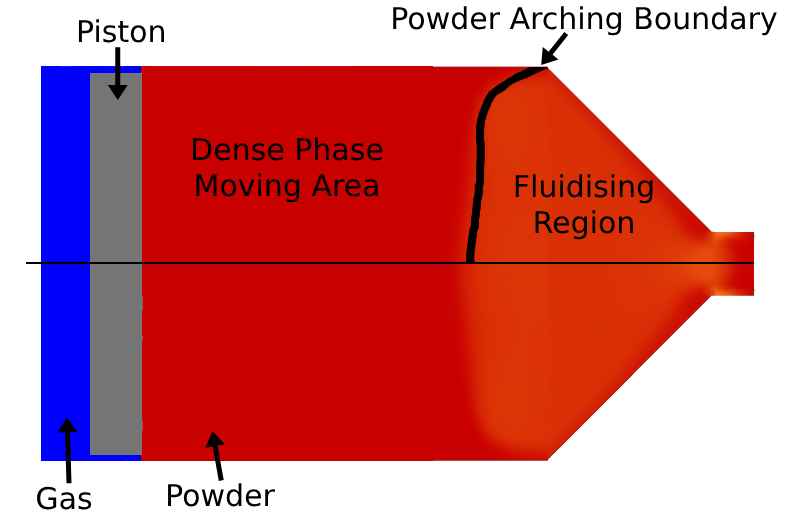
\includegraphics[width=\textwidth]{../report_assets/expected_result.png}
        \caption{Expected Behaviour}\label{fig:expected}
    \end{minipage}
    
\end{figure}
This analysis assumes arching occurs at the cone-tube interface, previously discussed in \autoref{sec:bulk-powder}, due to both geometric constriction and pressure applied by the piston. These conditions promote the formation of a stable arching structure that constrains powder flow. The model is further supported by two findings from literature. First, the piston velocity exhibits a linear relationship with the mass flow rate dispensed from the system~\cite{SUN201630}. Second, increasing the force on the piston initially raises the mass flow rate, but beyond a certain point this effect saturates, and further increases in piston force no longer lead to higher flow rates~\cite{LI2021712}.

Consider a scenario in which the piston provides minimal force on the powder. The fluidising region would then expand passed the cone-tube interface (leftwards on the diagram), similar to bed expansion. Applying greater piston force then would compress this region down, meaning a fluidising region with a higher density of powder. This would raise the number of particles close to the outlet and available for entrainment, resulting in a higher mass flow rate. If the piston force was increased further still, the fluidising region would compres down into the cone and the dense phase moving area would reach the cone-tube interface. At this point, arching occurs and any additional force from the piston is transferred through the powder column into the cone structure rather than compressing the fluidised region. This matches the behaviour reported in the literature, where increased piston pressure no longer increases the mass flow rate. 

This interpretation places places significant design constraints on the piston, which controls both the force exerted on the powder and the flow rate of fluidising gas. Both these are functions of the inlet pressure, and their coupling is non-trivial. While this interdependence complicates control, it also offers considerable advantages in terms of system miniaturisation, a trade-off considered acceptable within the scope of this design.

A second effect is also expected: a change in behaviour based on the amount of powder remaining in the tank. As discussed in \autoref{sec:background-powder-beds}, the pressure drop across a fluidised bed approximately equals the weight of the particles per unit area in the fluidised regime. Therefore, as the total powder mass decreases, so does the effective pressure drop, implying a dynamic relationship between powder quantity and the pressure experienced by the fluidising region.

\section{Experimental Setup}
The experimental set up was designed to verify the expected behaviour of the fluidising powder feed system under terrestrial conditions to better estimate it's behaviour under microgravity. The core aims were to record the consistency of the powder mass flow rate, verify that changing the pressure upstream of the tank leads to a change in mass flow rate and document any behaviours the system may exhibit that would impact it's suitability for space applications.

\subsection{Layout}
The default layout, seen in \autoref{fig:experimental-setup}, was used to perform most of the testing, with modifications outlined in the sections where they occur. 
\begin{figure}[htbp]
    \centering

    \begin{minipage}{0.6\textwidth}
        \centering
        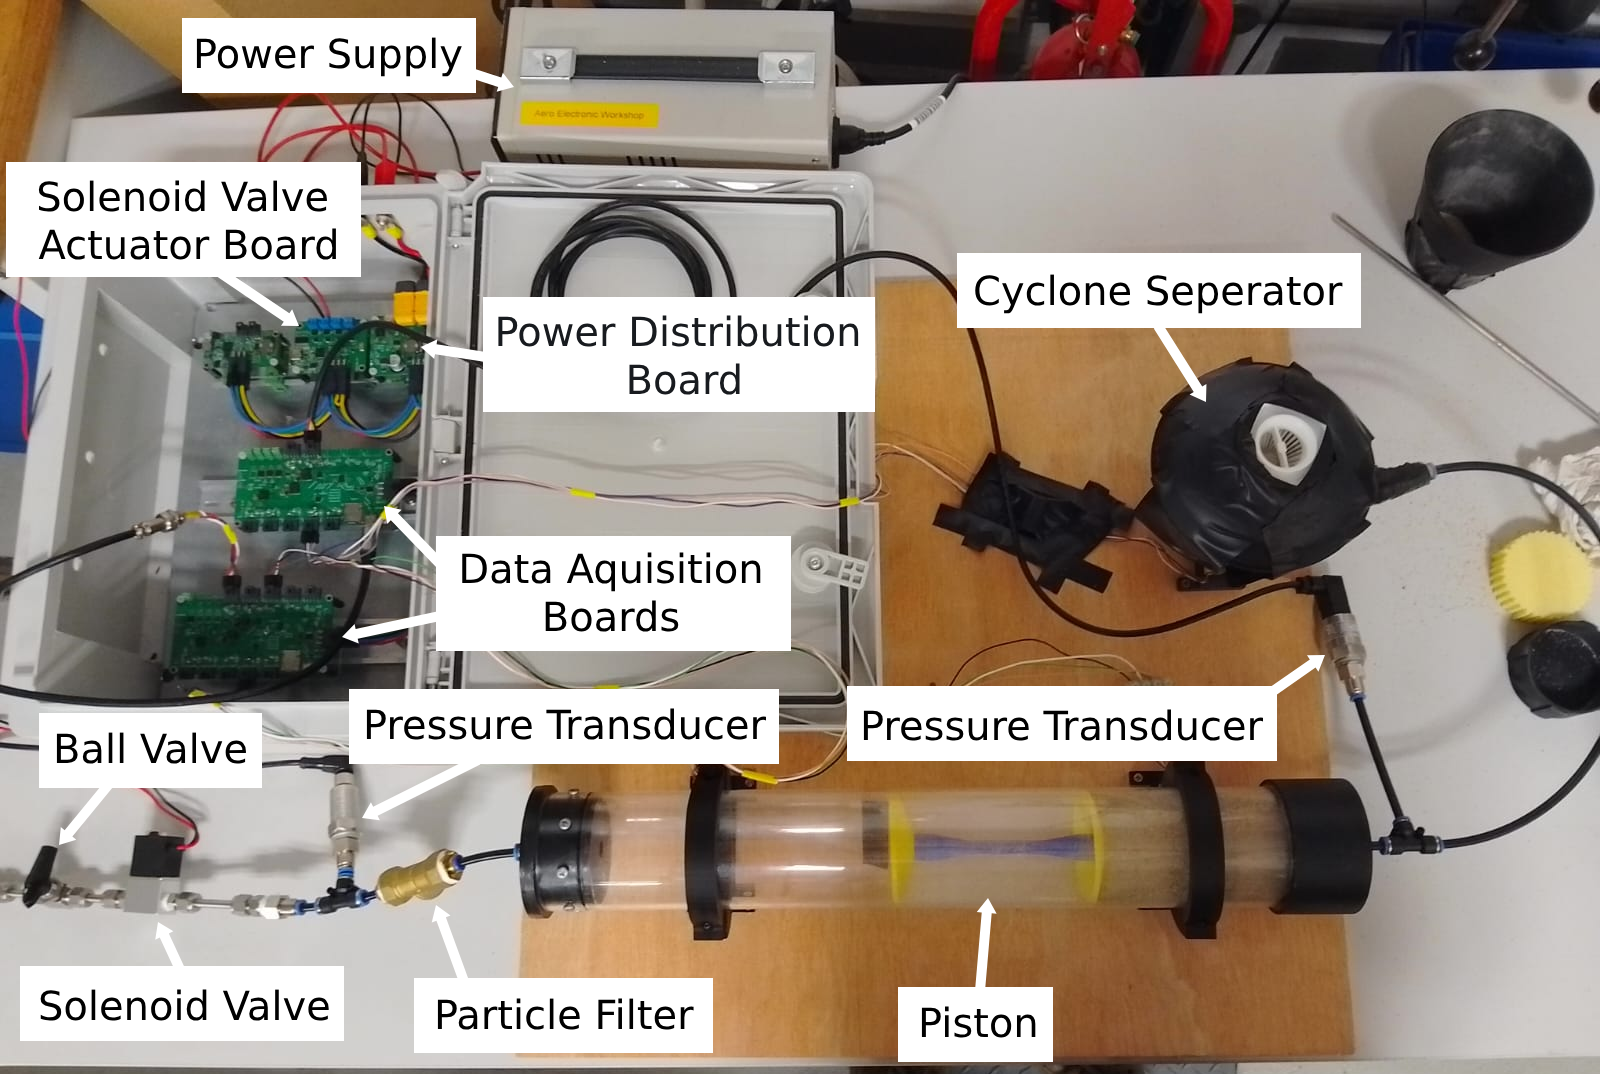
\includegraphics[width=\textwidth]{../report_assets/setup_annotated.png}
        \caption*{Annotated Image of Setup}
    \end{minipage}
    \hfill
    \begin{minipage}{0.3\textwidth}
        \centering
        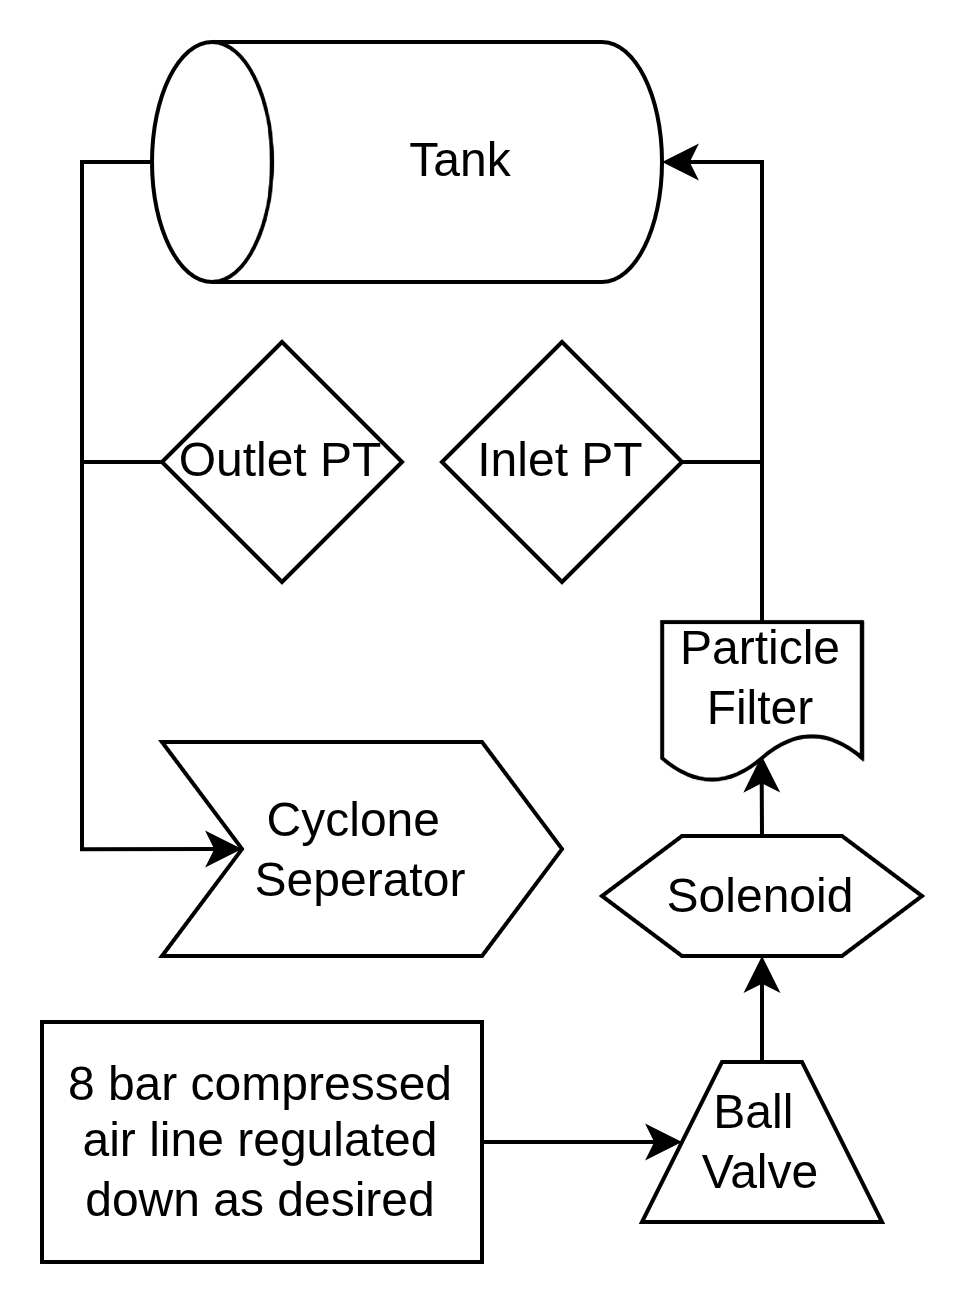
\includegraphics[width=\textwidth]{../report_assets/drawio_setup_vertical.png}
        \caption*{Systems Diagram of Setup}
    \end{minipage}
    \caption{Experimental Setup}\label{fig:experimental-setup}
\end{figure}
Testing was conducted in Imperial College's Hypersonic Laboratory, which does not have climate control. It was assumed that the system would not behave noticeably differently under the slight variations in temperature and pressure that occurred during the testing period.

\subsection{Data Acquisition and System Actuation}
To capture the system's behaviour, a combination of video recordings, load cell readings and pressure transducer readings were taken during each test. The placement of the sensors is shown in \autoref{fig:sensors} and their values were read with the use of custom electronics designed by the Imperial College London Rocketry team.
\begin{figure}[htbp]
    \centering

    \begin{minipage}{0.45\textwidth}
        \centering
        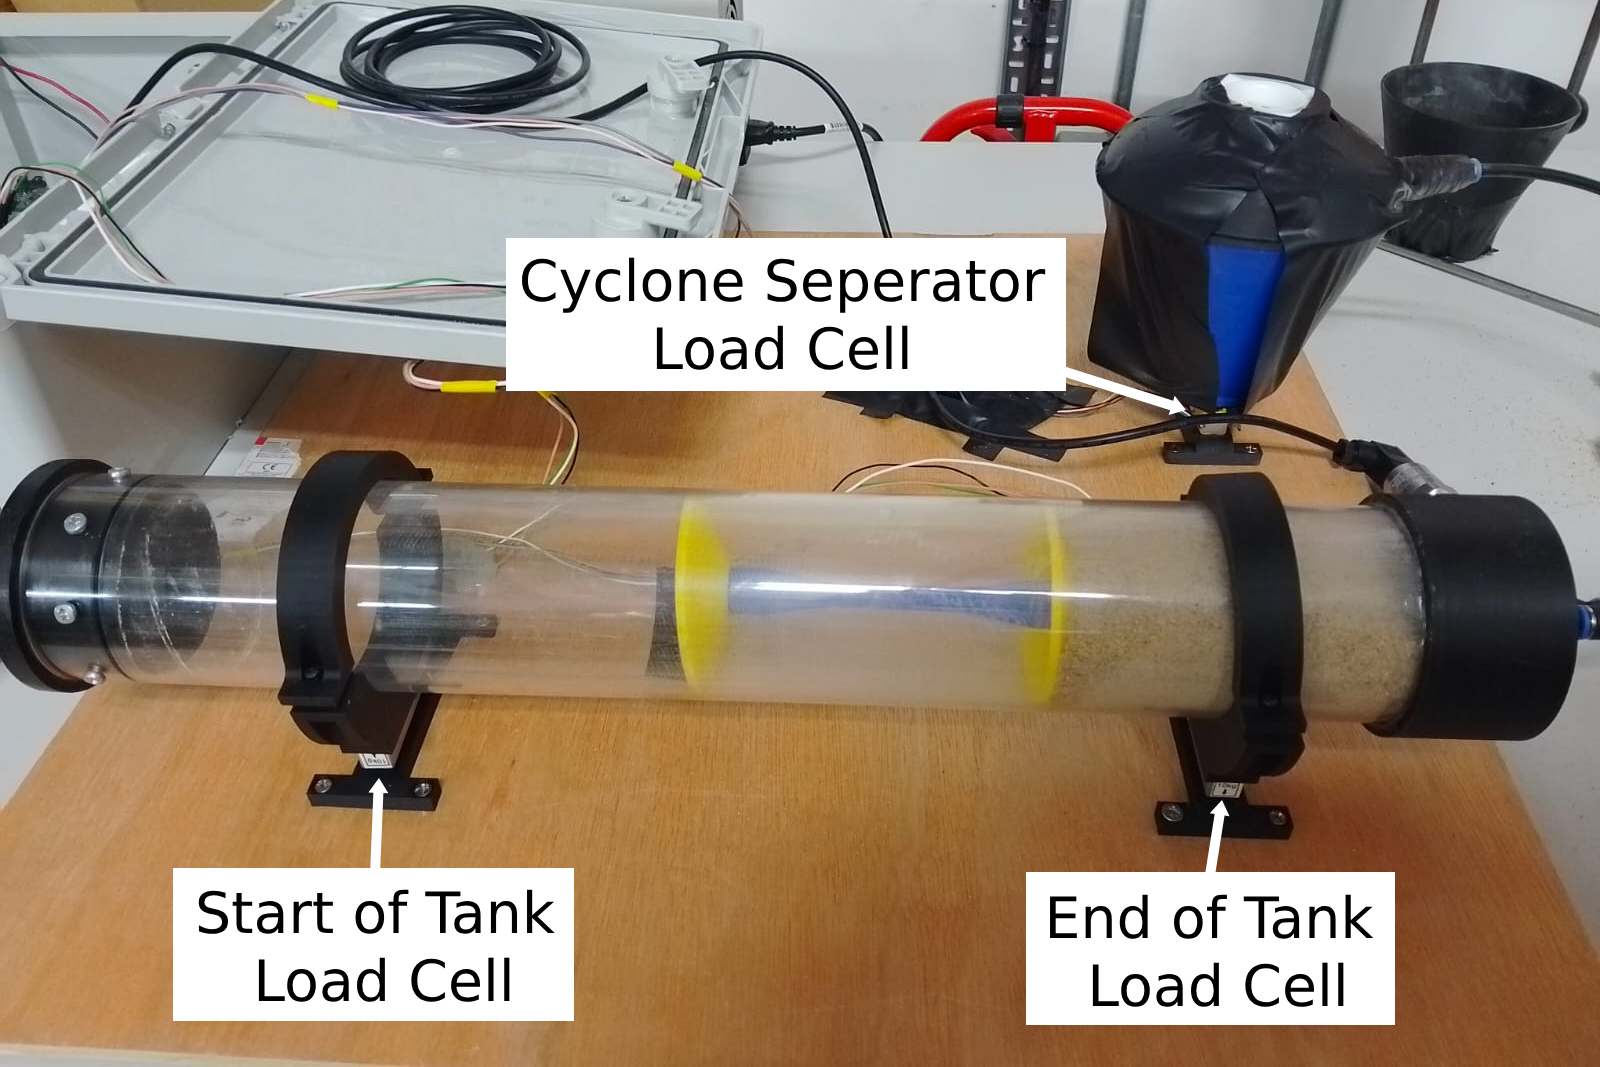
\includegraphics[width=\textwidth]{../report_assets/load_cell_configuration.png}
        \caption*{Load Cell Placement}
    \end{minipage}
    \hfill
    \begin{minipage}{0.45\textwidth}
        \centering
        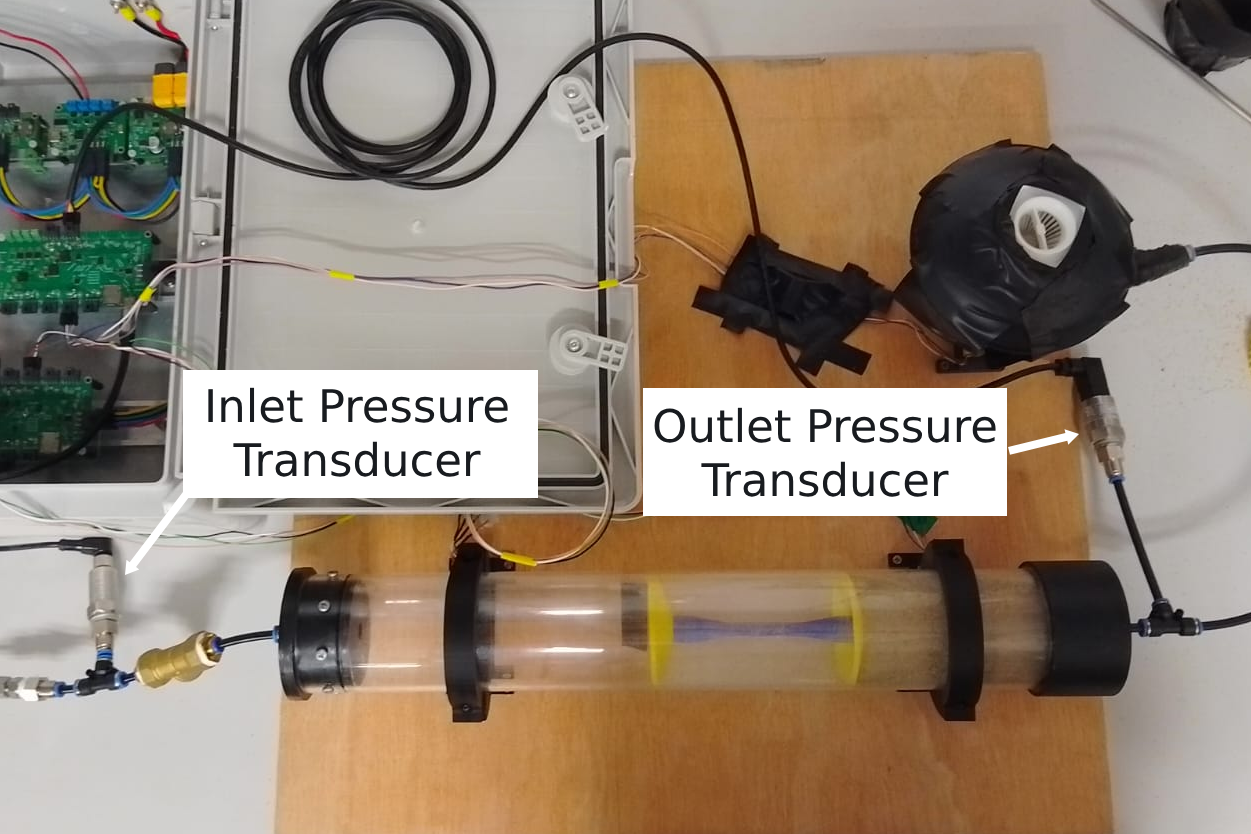
\includegraphics[width=\textwidth]{../report_assets/pressure_transducer_configuration.png}
        \caption*{Pressure Transducer Placement}
    \end{minipage}
    \caption{Sensor Placement in Experimental Setup}\label{fig:sensors}
\end{figure}
The load cells were placed at the start and end of the tank as well as beneath the cyclone separator. This was done as it allows for two independent measurements of powder mass movement to allow for cross-validation and redundancy. The pressure transducers were placed before and after the tank with the goal of being able to use them for a deeper analysis of the system. This analysis was never conducted due to the complexity of modelling the pistons impact on the static pressure as well as time constraints of the project.

A computer was connected to the electronics system to log and display the data on a bespoke user interface, shown in \autoref{fig:grafana}. The solenoid valve, seen in \autoref{fig:experimental-setup}, could also be opened and closed through the dashboard, allowing for safe operation as all the information and control was in one place.
\begin{figure}[htbp]
    \centering

    \begin{minipage}{0.95\textwidth}
        \centering
        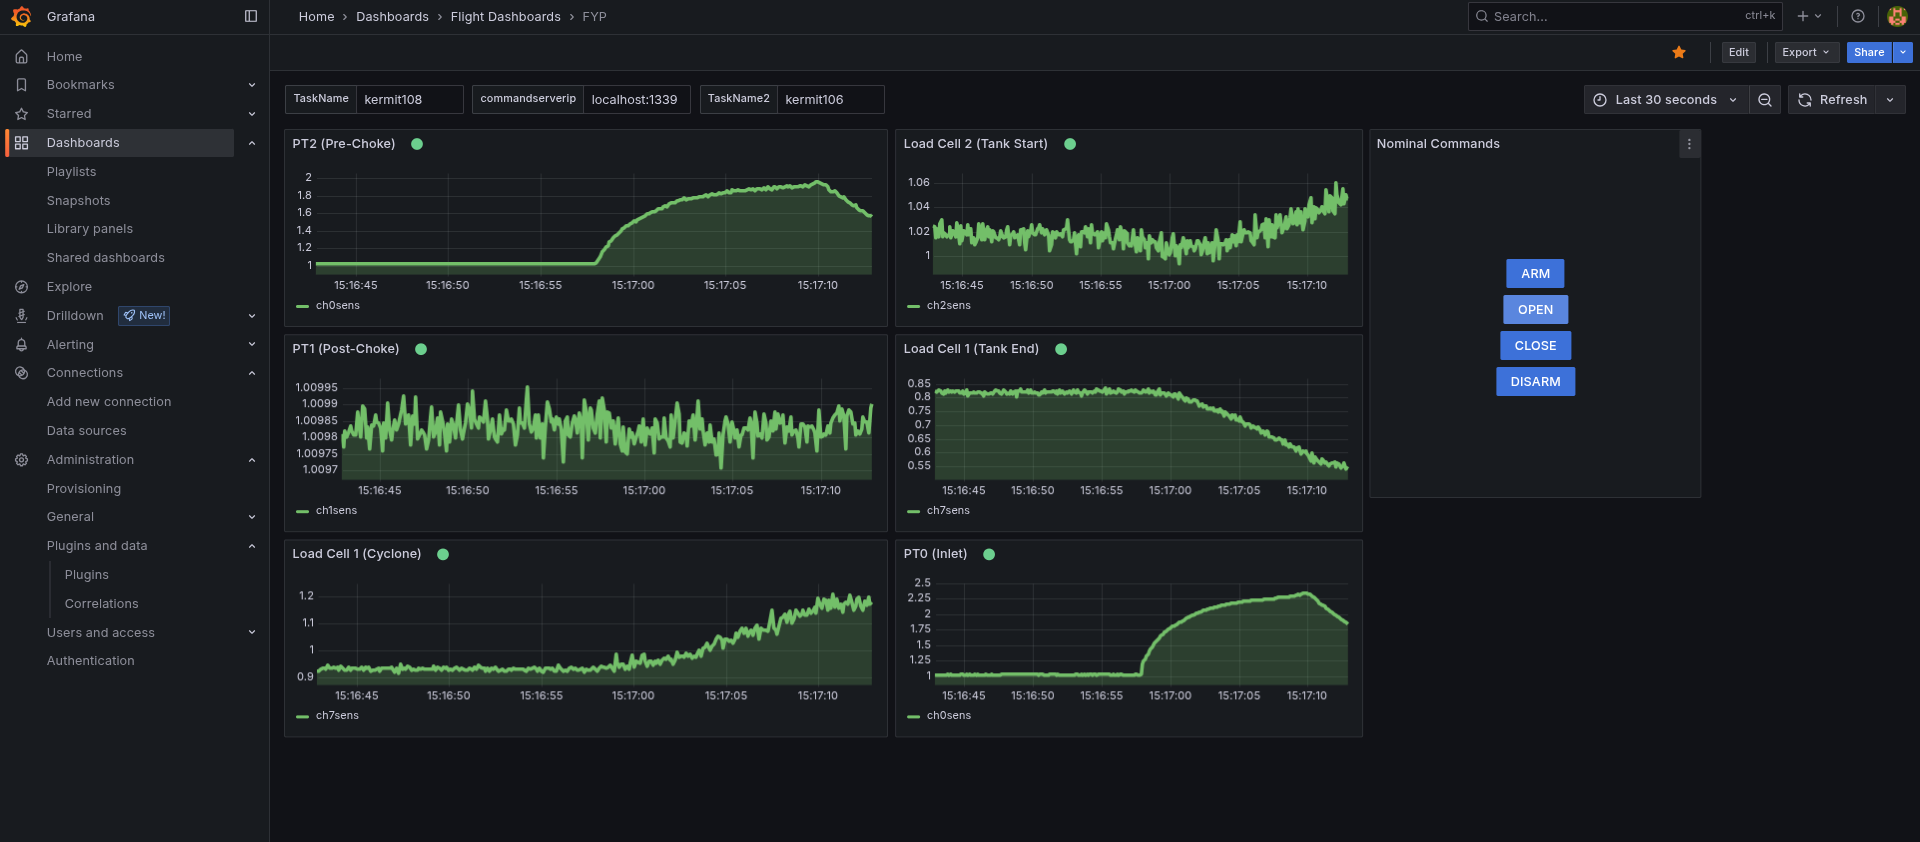
\includegraphics[width=\textwidth]{../report_assets/grafana.png}
        \caption{Testing Dashboard}\label{fig:grafana}
    \end{minipage}

\end{figure}
Due to budget constraints, low-cost pressure transducers and load cells were used. Given this, extensive calibration was not prioritised as these components typically exhibit higher variability and lower stability, limiting the benefits of precise calibration. To calibrate the load cells, the data aquisition board was configured to record the raw values output by the analog to digital converter (ADC) at both the unloaded, 0kg, state and then with a mass, measured at 0.746kg, placed on it. Since the load cells are a linear sensor, these two points give a gradient and y-intercept to map the ADC counts to. The same procedure was done to calibrate the pressure transducers except using a mechanical pressure gauge and the compressed air line to record 1 bar and 4 bar ADC outputs.

An older setup of the experiment included a choke point just after the outlet of the tank. This was because previous literature proposed that fluidising systems where one part of the gas-solid flow is in choking conditions had been found to be simpler to control~\cite{SUN201630}. Due to the grain size of the sand, this chokepoint got clogged in testing so was removed. As there was a pressure transducer before and after the chokepoint, this explains the data labels in \autoref{fig:grafana} and why the pre-choke pressure data is just noise as it was no longer connected.

\subsection{Cyclone Separator and Measurement Method}
The two most common methods of measuring mass flow rate for this kind of system are using a displacement transducer to measure how far down the tank the piston is or measuring the mass of the powder after it has been fed out of the tank~\cite{SUN201630}\cite{LI2021712}\cite{Tang22}. The displacement transducer method indirectly measures the mass flow by using the near incompressibility of the powder and the assumption of a constant packing density to form a linear relationship between the movement of the piston and the volume of powder dispensed~\cite{SUN201630}. The direct method requires some method of seperating the gas and powder after it has exited the system and then measures the mass of powder over time. 

The direct mass measurement method was used as it had multiple advantages over measuring piston displacement. The first being there was no additional modifications to the tank end cap needed as to incorporate the a displacement transducer, a hole would have to be drilled and could provide another place for leaks to occur. If any powder found it's way behind the piston it could interfere with the displacement readings and there is a risk that the piston velocity would not be constant, a concern that was validated during testing. Finally, the powder needed to be contained no matter what method was chosen as airbourne sand particles are a hazard to lung health so adding a load cell to this containment method was much easier to implement.

To contain the powder and seperate out the gas, a cyclone separator was used, seen in \autoref{fig:cyclone}.
\begin{figure}[htbp]
    \centering

    \begin{minipage}{0.3\textwidth}
        \centering
        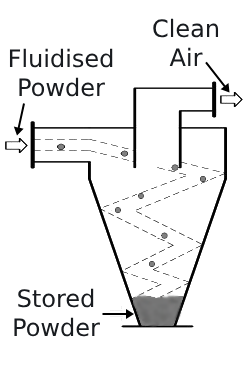
\includegraphics[width=\textwidth]{../report_assets/cyclone_diagram.png}
        \caption*{(a) Cyclone Separator Diagram}
    \end{minipage}
    \hfill
    \begin{minipage}{0.3\textwidth}
        \centering
        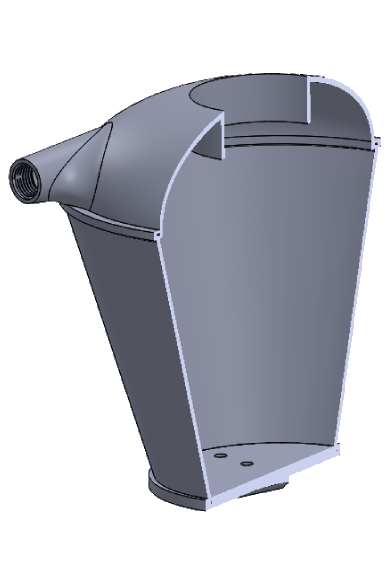
\includegraphics[width=\textwidth]{../report_assets/cyclone_cad.png}
        \caption*{(b) CAD Model of Separator}
    \end{minipage}
    \hfill
    \begin{minipage}{0.3\textwidth}
        \centering
        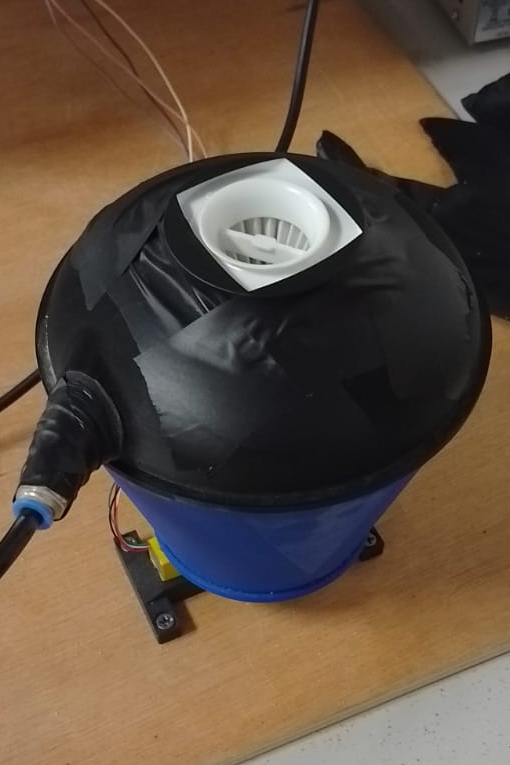
\includegraphics[width=\textwidth]{../report_assets/cyclone_done.png}
        \caption*{(c) Cyclone Separator}
    \end{minipage}
    \caption{Sensor Placement in Experimental Setup}\label{fig:cyclone}
\end{figure}
A cyclone separator works by using centrifugal force to separate the sand from the air. As the mixture enters the cyclone chamber tangentially at high speed, it spins rapidly, causing the denser particles to move outward and fall to the bottom, while the cleaner air exits through the top center. As shown in \autoref{fig:cyclone} (c), a dust filter used in vacuum cleaners was used to ensure any fine grains, not captured by the separator, do not make it out into the air. This was attached to the 3D printed model using PTFE tape and a friction fit, then taped down for added support. The separator was printed in 3 parts, the top that can be removed to empty out the sand, the walls and the base with screw holes to mount to the load cell.
% The direct cyclone separator method was chosen to record mass flow, with a back up recording of the mass of the tank during operations. This is because the sand needs to be contained after exiting the tank as inhalation of silica particles can lead to long term health conditions. Therefore, the direct method was chosen as

\subsection{Powder}
While typical powders used in CSAM are $5\,\mu\mathrm{m}$ to $100\,\mu\mathrm{m}$~\cite{Vaz2023}, budget constraints resulted in sand being the optimal granular material safe enough to work with. This will definitely affect the behaviour of the system but to what extent is unknown. A rudimentary attempt was made to measure the particle diameter using a micrometer but given the time limitations, no formal attempt was made to characterise the diameter distributions or average diameter. As mentioned in \autoref{sec:numerical-setup}, the bulk density, that being the density of the sand including the volume occupied by air, was measured by recording the mass of the sand in a bowl and then filling the same bowl with water.

% For safety and due to the limited budget, sand was used as the powder. This is one of the greatest areas for improvement, i dont actually know what size the powder is or the distribution of those sizes. This powder has been measured to have [density = 1.4g/cm3]

% \newpage

\subsection{Procedure to Characterise Pressure Source}\label{sec:pressure-source-procedure}
Due to safety and ease of handling, the pressurised air supplied into the system came from a compressed air line. As mentioned in \autoref{sec:first-test}, the pressure readings from preliminary testing were lower than expected so an attempt at characterising the air supply was made. 

To do this, the steady-state flow through the system without any piston or sand was investigated by measuring the static pressure before and after the tank at different regulator settings. Tuning of the regulator was consistent across all experiments conducted and was done as follows. The system was closed by replacing the inlet pipe into the tank with a pushfit end cap, as seen in figure \autoref{fig:systems-diagram-end-cap}.
\begin{figure}[htbp]
    \centering
    \begin{minipage}{0.60\textwidth}
        \centering
        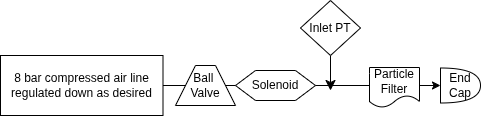
\includegraphics[width=\textwidth]{../report_assets/end_cap.drawio.png}
        \caption{System Diagram of Closed System}\label{fig:systems-diagram-end-cap}
    \end{minipage}
\end{figure}
The regulator integrated into the compressed air line was then adjusted using the inlet pressure transducer readings as a reference. While there was a gauge on the regulator, it was consistently reading 0.2 to 0.3 bar higher than the pressure transducers in the system or manual pressure gauges used and was therefore deemed unreliable. Once the pressure was tuned on the regulator, the valves were closed, the end cap was removed and the tube was reattached to the tank, returning to the default configuration. 

Confirmation of the lower than expected static pressure readings motivated follow-up tests to eliminate possible sources of human error in the system setup. The pressure regulator integrated into the compressed air line was checked first by including another gauge closer to the system and fully opening the integrated one. If the static pressure losses were because of the 2 metres of nylon tube from the air line to the experimental setup, this would also have been highlighted.

Additionally, the solenoid valve could have had a very small orifice area, potentially choking the flow just before the pressure transducer. To test this, the valve was removed, and additional tests were conducted with the component excluded.

\subsection{Procedure to Characterise Full System}
To ensure an equal comparison between the behaviour of the system at different inlet pressure configurations, a consistent testing procedure was adhered to.

Starting from default configuration with nothing in the tank clean tank, the inlet end cap was removed and the piston was placed in it. This was positioned at the start of the tank to lower the chance that the piston gets stuck on the sand that forms an incline, seen in \autoref{fig:sand-ramp}.
\begin{figure}[htbp]
    \centering
    
    \begin{minipage}{0.60\textwidth}
        \centering
        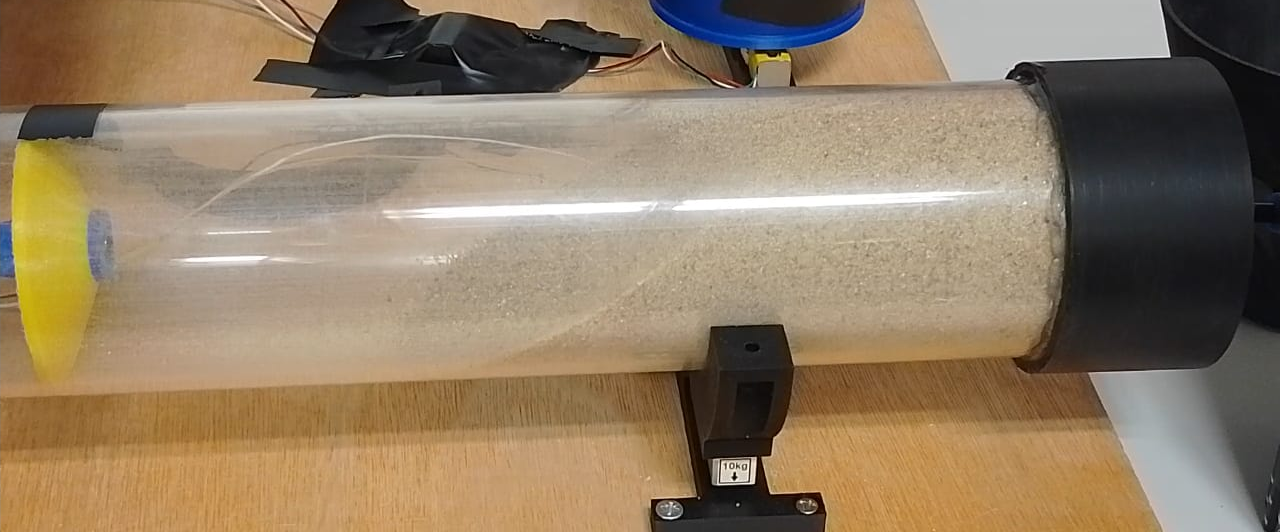
\includegraphics[width=\textwidth]{../report_assets/sand_ramp.png}
        \caption{Starting Sand Distribution in Tank}\label{fig:sand-ramp}
    \end{minipage}

\end{figure}
If the piston has time to accelerate from far away, it was found to be more likely to sweep that ramp sand forwards with its movement and fully pack the sand into the outlet instead of getting stuck. Next the female pushfit fitting was removed from the outlet of the tank and 1000 g to 1020 g of sand was measured out and put into the tank through the use of a funnel. Once the sand had filled the tank, the pushfit fitting was reattached and a tube with an end cap was placed over the outlet. The tank was then held vertically such that the outlet was facing down and tapped to ensure no sand was stuck to the walls close to the piston, preventing successful startup. Then the tank was placed on the load cell stands, ensuring that the system starts with sand fully covering the cross section of the tank close to the outlet, again seen in \autoref{fig:sand-ramp}. Once placed down, the end cap tube was removed from the inlet and the tube leading to the cyclone separator was connected. The cyclone separator was then taped down to reduce the likelihood the lid pops off. It is thought that this was only necessary due to the undersizing of the cyclone separator but since taping it solved the issue, a 3rd iteration on the design was deemed unnecessary. Once the system was set up, the pressure regulator was tuned like in \autoref{sec:pressure-source-procedure}. End cap was removed from the closed system configuration and the tube was then reattached to the tank inlet.

Now that the system was ready for testing the valves were opened and the data was logged. Ideally, the computer would have been placed far away from the system, the ball valve would have been opened and only when the solenoid valve was actuated remotely would the system function. Unfortunately, due to the solenoid valve leaking, the computer had to be placed near the system to minimise the time between opening the ball valve and actuating the solenoid. Once the pressure reading at the outlet had dropped sufficiently, it was assumed all the powder had been dispensed into the separator and the valves were closed.

\section{Numerical Setup}\label{sec:numerical-setup}
\subsection{Numerical Setup to Characterise Pressure Source}
To provide an additional angle into the investigation of source pressure behaviour, seen in \autoref{sec:static_test}, an axisymmetric simulation was conducted of the system without a piston or powder in the tank. The geometry used can be seen in \autoref{fig:geometry_static_sim}, noting the two vertices in the geometry outlined to record the numerical values of pressure at locations similar to the pressure transducers in the experimental setup.
\begin{figure}[htbp]
    \centering
    
    \begin{minipage}{0.9\textwidth}
        \centering
        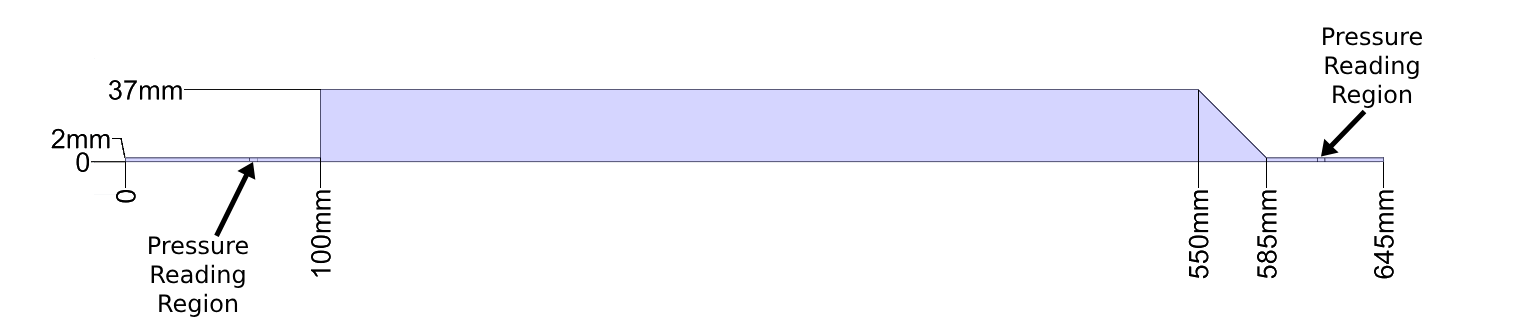
\includegraphics[width=\textwidth]{../report_assets/geom_pressure_losses.png}
        \caption{Geometry of Simulation to Characterise Pressure Source}\label{fig:geometry_static_sim}
    \end{minipage}
    
\end{figure}
An axisymmetric model was chosen as it requires far fewer computations due to the lower number of cells, while still preserving the pressure quantities of the 3D physics. This was possible as it is expected that there would be no angular dependence around the axis of revolution and no swirling is expected to occur. Because of the reduced time requirement of the axisymmetric model, the mesh used 0.1mm square cells to produce a high resolution analysis of the flow. The inlet was modelled as a pressure inlet with a stagnation pressure of 2 bar and the outlet was a pressure outlet at atmospheric conditions. The gas used was air under standard operating conditions as this assumed to be close to what is output from the compressed air line.
\subsection{Numerical Setup to Characterise Full System}
To investigate how well the design would translate to the space environment, numerical simulations to observe key flow features were conducted. Given that there is no experimental data on fluidisation under microgravity present in literature, options to verify the validity of the simulations are limited. Therefore, attempts to show well documented behaviours like the relationship between piston velocity and mass flow rate were made. Anchoring the validitiy in these relationships given no other options. The scope of the project reduced the simulation methods to pre-existing software and Ansys Fluent was chosen as it could perform moving mesh simulations as well as two phase flow simulations with limited prerequisit knowledge.

Given the complexity of the simulation, an extensive testing campaign was undertaken with only the final simulation outlined below. The simulation software chosen has a limit on the number of cells a mesh can have when using the student license. This restricted the modelling options to axisymmetric and 2D. Given that gravity is not an axisymmetric phenomenon and the tank was oriented horizontally in experiments to limit the affect of gravity on the system, a 2D simulation was conducted. 

Experimentation with the mesh found that 1mm squares was optimal with respect to simulation stability and run time. A time step of 0.0001s was used meaning only timeframes were analysed but this 
\begin{figure}[htbp]
    \centering

    \begin{minipage}{0.45\textwidth}
        \centering
        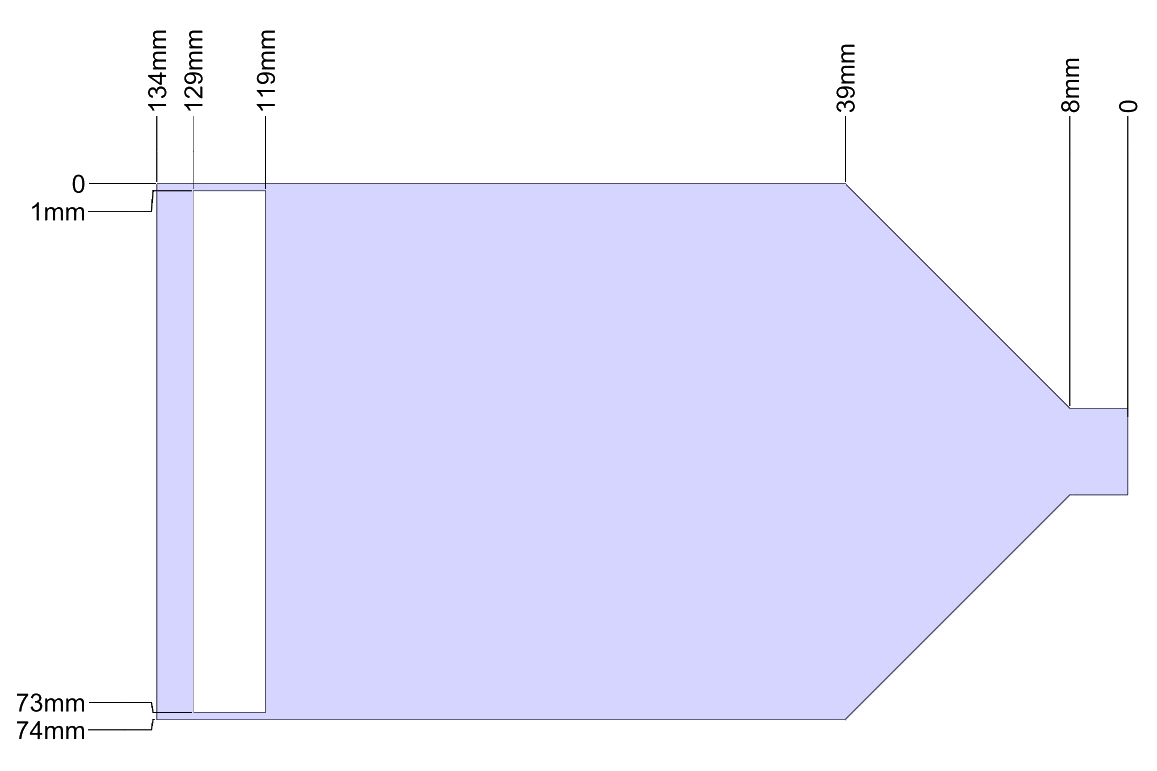
\includegraphics[width=\textwidth]{../report_assets/big_sim_geom.png}
        \caption{2D Geometry of Tank}\label{fig:2D-tank}
    \end{minipage}
    \hfill
    \begin{minipage}{0.45\textwidth}
        \centering
        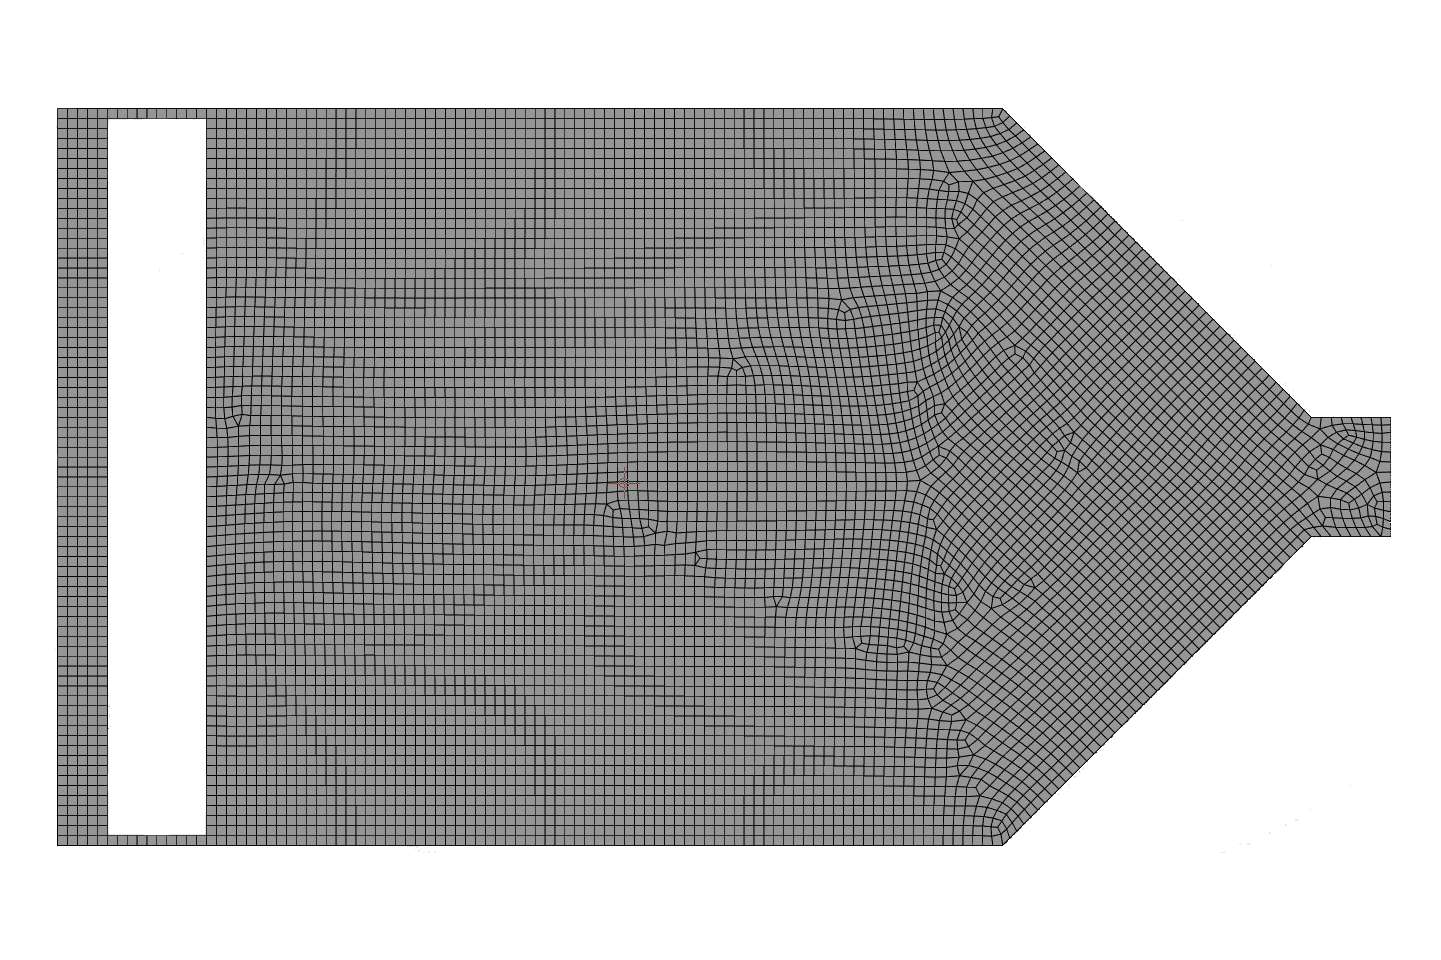
\includegraphics[width=\textwidth]{../report_assets/big_sim_mesh.png}
        \caption{Mesh of Tank}\label{fig:mesh-tank}
    \end{minipage}

\end{figure}
The simulations were underpinned by two mechanisms, both add significant complexity to the simulations. The first is the two-phase aspect of the simulations. 

The second is the fluid structure interactions present with the moving mesh.


at first, the moving mesh just deleted the powder instead of pushing it, to solve this problem
granular temperature was investigated

a second set up was then created to run smaller tests investigating the movement of powder
frictional packing was then added as the pow

after this started working, it was then transferred to the mesh shown above where another issue of dynamic remeshing occured

after figuring out this was a limitation placed on the student license, smoothing and the other one were used and the system not crashing was just hoped for

\begin{figure}[htbp]
    \centering

    \begin{minipage}{0.45\textwidth}
        \centering
        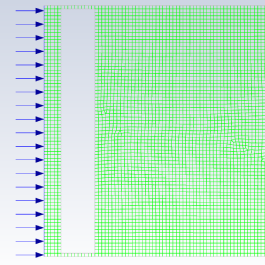
\includegraphics[width=\textwidth]{../report_assets/mesh_before_moving.png}
        \caption{Mesh at Beginning of Simulation}\label{fig:beginning-mesh}
    \end{minipage}
    \hfill
    \begin{minipage}{0.45\textwidth}
        \centering
        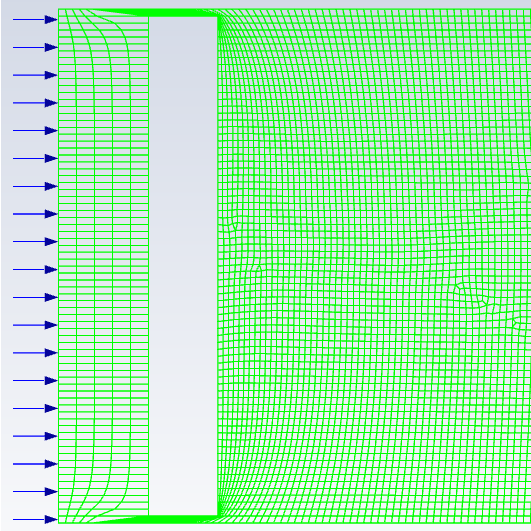
\includegraphics[width=\textwidth]{../report_assets/mesh_after_moving.png}
        \caption{Mesh at End of Simulation}\label{fig:end-mesh}
    \end{minipage}

\end{figure}
obviously not ideal but no other option

next the simulation was ran under zero gravity as this was simpler to implement, crashing happened at different times in the simulation based on the speed of the piston so it is thought to be because of the meshing problem

when gravity was turned on the simulation crashed even faster, this is thought to be because the powder packs down to the bottom and then the piston is trying to push powder that cannot compress anymore creating physical instabilities

















% \subsection{Moving piston simulation}
% governing equations eularian-eularian
% 2d is valid because:
% 2D vs 3D Eulerian Multiphase Simulations of a Piston-Driven Fluidised Bed
% Flow Features in 2D vs 3D Multiphase Models
% Hydrodynamics and Void Distribution: Two-dimensional Eulerian-Eulerian simulations can reproduce many qualitative behaviors of fluidised beds, but they often differ quantitatively from three-dimensional models. A key issue is that 2D models tend to over-predict void fractions and bed expansion, especially at higher flow velocities
% link.springer.com
% . This occurs because neglecting the third dimension forces the gas-solid flow into a constrained plane, which exaggerates hydrodynamic structures and fluctuations
% link.springer.com
% . In practical terms, a 2D simulation may show larger void regions (bubbles) and more vigorous oscillations in solid concentration than a real 3D system would. These differences mean that certain flow features are not identical between 2D and 3D:Bubble Dynamics: Gas bubbles in a fluidised bed behave differently in a 2D domain. Studies have found that bubbles remain smaller and rise more slowly in a 2D (pseudo-2D) bed than in a full 3D bed
% witpress.com
% . In a 3D simulation or experiment, bubbles can expand and coalesce in three directions, forming larger voids that accelerate upward. The 2D constraint suppresses some coalescence, so the bed may appear “bubblier” (many small bubbles) or even form slugging bubbles that span the width. This impacts particle motion and could alter the paths through which solids circulate and exit the bed.
% Circulation and Wall Effects: Three-dimensional beds allow complex circulation patterns — particles can move around bubbles and across the entire cross-section. In a 2D model, by contrast, flow is essentially confined between two parallel walls (the front and back of the 2D slice). This artificial confinement increases wall friction effects and creates a large circulating cell in the 2D plane that has no out-of-plane escape. As a result, 2D simulations may produce stronger single circulation loops or jetting along the centerline, whereas a 3D bed would have more distributed flow paths (including around the perimeter of bubbles or toward the center of a cylinder). Such differences could influence how continuously and evenly the powder flows out — 3D systems tend to have more uniform, axisymmetric flow, while 2D systems might exhibit more pronounced channeling or periodic “puffing.”
% Turbulence and Mixing: The restriction to two dimensions also affects turbulence and mixing of the phases. Fully 3D turbulent eddies and clusters cannot form in a 2D plane, so 2D simulations often show greater oscillatory behavior (numerical instability or large-scale swings) but less of the small-scale chaotic mixing present in 3D
% link.springer.com
% . For example, pressure fluctuation spectra differ: only a 3D simulation can capture realistic pressure dynamics, whereas a 2D model gives a distorted spectrum
% witpress.com
% . This means the distribution of particles and the stability of the fluidization can differ — a 3D bed might self-buffer some fluctuations by distributing them in all directions, while a 2D bed tends to amplify fluctuations within its constrained geometry.
% Implications for Mass Flow Features: These flow-feature disparities imply that certain phenomena affecting mass outflow could differ between 2D and 3D. For instance, jetting and channeling of powder-gas mixture might be more pronounced in one case versus the other. A 3D piston-driven bed could develop a roughly axisymmetric flow of powder out of the piston region, whereas a 2D model might produce a sheet-like ejection that interacts differently with the walls. Likewise, particle distribution in 3D may be more uniform across the cross-section of an outlet, while in 2D it might be clumped or stratified, potentially affecting instantaneous mass flow rates. Overall, 2D models capture the qualitative flow patterns (e.g.fluidization regimes, general trends in circulation), but certain 3D-specific effects (like true spatial distribution of particles, or the full spectrum of bubble sizes) are lost, which can influence the accuracy of mass flow predictions
% witpress.com
% witpress.com
% . Researchers therefore caution that 2D CFD results should be used primarily for sensitivity studies or trend analysis, whereas 3D simulations are needed to accurately reproduce absolute measures like bed expansion, bubble size distributions, and pressure oscillation characteristics
% witpress.com
% witpress.com
% . In short, 2D and 3D models can differ in circulation patterns, particle clustering, wall friction effects and turbulence - all of which may affect the steady powder outflow rate.
% Linearity of Piston Velocity vs. Powder Mass Flow Rate
% Experimental Observation: In piston-driven fluidised beds (such as pneumatic powder feeders or powder-fueled engines), experiments consistently show that the powder mass flow rate increases approximately linearly with piston velocity (or with related parameters like the throttle/orifice opening)
% researchgate.net
% . Essentially, driving the piston faster injects a larger volume of gas-solids mixture per unit time, yielding a higher mass flow. This linear relationship holds as long as the system is operating below any choking or saturation limits. For example, one study of a powder fuel feeding system found a “high linear tendency” between the mass flow rate and the minimum throttle area (which correlates with piston drive conditions), within the tested range
% researchgate.net
% . Such linear scaling is a fundamental expectation for a displacement-driven flow. 2D Simulation vs 3D Reality: A well-configured 2D Eulerian-Eulerian simulation should qualitatively preserve this linear trend. If the piston (modeled perhaps as a moving wall or boundary in Fluent) is run at different velocities in a 2D model, one would observe that the outflow of powder increases proportionally. In fact, simplified models often treat the piston-induced flow like a controlled volumetric flow rate, which inherently is linear with piston speed in the absence of complex losses. The key question is accuracy: whether the 2D model’s slope of the mass flow vs. velocity curve matches that of a real 3D system. Geometric constraints can introduce some error here. For instance, 2D simulations, by overestimating void fraction and ease of fluidization, might predict slightly higher mass flow for a given piston speed than a 3D simulation or experiment would
% link.springer.com
% . This is because the 2D model may fluidize the powder bed more readily (bubbles percolating easily in the planar slice), offering less resistance to the piston. On the other hand, certain flow resistances (like friction along side walls or limitations in cross-sectional expansion) in 2D could also cause underestimation in some regimes. Notably, discrepancies are expected to grow at more extreme velocities or flow rates. Xie et al. found that when gas velocities are high, the divergence between 2D and 3D models becomes significant - 2D could not satisfactorily predict the hydrodynamics observed in a 3D cylindrical bed
% link.springer.com
% . By contrast, at lower velocities (milder fluidization), 2D and 3D results were more similar
% link.springer.com
% . Translating this to a piston-driven scenario: at modest piston speeds (near the linear operating regime), a 2D simulation will likely yield a linear mass flow response very close to reality. However, as piston velocity increases (approaching choking flow or very aggressive fluidization), the 2D model might deviate - for example, it might fail to capture the onset of non-linearity or throughput limitations that a 3D system would experience. Real 3D systems can develop complex flow distribution (e.g. some regions flowing while others channel or form stagnant zones) at high rates, whereas a 2D model may either over-homogenize this or exhibit unphysical oscillations. Thus, while the linear relationship itself is likely to appear in 2D simulations, the fidelity of its slope and any departure at extremes must be treated with caution. Validation against 3D data or correlations is advised if one plans to use 2D results for quantitative predictions of mass flow.
% Reliability of 2D Predictions and Use in Design
% Early-Stage Design Use: Despite their limitations, 2D multiphase simulations are widely used in early design and feasibility studies because they are much less computationally intensive than 3D models. Importantly, they capture the basic trends and physics of the system, which is often sufficient for preliminary performance estimates. As noted in a recent review, for certain applications like preliminary thermodynamic design or scouting different operating conditions, the more complex 3D approach “does not offer significant benefits” over 2D in terms of high-level outcomes
% link.springer.com
% . The core behaviors - e.g. how increased piston speed affects flow, or how changes in gas feed influence fluidization - are reflected reasonably well in 2D. In fact, 2D simulations can be effectively utilized to illustrate behavioral trends, albeit with some “acceptable disadvantages” such as misrepresentation of exact bed expansion
% link.springer.com
% . In the context of a piston-driven powder bed, a 2D Fluent model would be a theoretically sound and practically convenient tool to predict whether, say, doubling the piston velocity doubles the powder delivery rate (and it likely will show that linear doubling trend). This helps an engineer get a quick sense of performance scaling without the overhead of a full 3D simulation. Known Limitations: However, one should not take 2D results as gospel when it comes to absolute performance or detailed flow behavior. Multiple validation studies have concluded that 2D simulations should be used with caution and primarily for qualitative insight or sensitivity analysis
% witpress.com
% witpress.com
% . They are not fully predictive of 3D behavior in a quantitative sense. For example, a 2D model might predict a certain mass flow rate for a given piston speed that differs from the real 3D value by a noticeable margin (due to differences in void fraction and wall friction effects). It might also fail to predict phenomena like unequal powder distribution in a 3D hopper, or the exact point where increasing piston velocity no longer yields proportional increases (onset of choking). As one study put it, only a 3D simulation was able to reproduce both the correct bed height and the dynamic pressure fluctuations of a bubbling bed, whereas 2D had significant deviations
% witpress.com
% . Conclusion - “Acceptable with Caution”: For the piston-driven fluidised bed scenario, using a 2D Eulerian-Eulerian Fluent simulation is reasonable in the early project stages. It offers a fast and informative approximation, and it will likely correctly indicate that there is a linear relationship between piston speed and powder mass flow under normal operating conditions. This makes it a practically acceptable tool for initial design and performance prediction. The literature supports this usage: 2D models can reliably rank design options and reveal trends (e.g. that higher piston speeds yield proportionally higher flow)
% researchgate.net
% , and they can guide engineers on what range of operation is plausible. The theoretical basis (continuity and momentum balance of two-phase flow) is sound, so there is no fundamental reason the 2D model would invert or lose the linear trend. What must be kept in mind is that extrapolating 2D results to 3D comes with uncertainty. Engineers should apply conservative corrections or eventually verify with a 3D model or experiments. In early design, one might use 2D to narrow the design space (thanks to its speed), then use a higher-fidelity 3D simulation on the shortlisted cases. By doing so, one benefits from the strengths of both approaches. In summary, 2D Eulerian-Eulerian simulations are theoretically sound for capturing the essential flow physics and trends of a piston-driven powder bed, and they are practically very useful in the initial design phase. They do preserve the linear piston velocity vs. mass flow relationship observed in 3D
% researchgate.net
% . Yet, because of geometric constraints, they can introduce errors in flow details and magnitudes, so their predictions should be regarded as preliminary. For final design confidence - especially if subtle 3D flow features (circulation patterns, non-uniform outflow, etc.) matter - a 3D simulation or experimental validation is recommended
% witpress.com
% link.springer.com
% . The consensus in the literature is that 2D and 3D approaches complement each other: use 2D for efficiency and scoping, and 3D for accuracy and final verification
% link.springer.com
% witpress.com
% . Sources: Recent computational studies and reviews of fluidised bed modeling and pneumatic powder feeding have informed these conclusions. Notably, comparisons by Yılmaz et al. (2025) on 2D vs 3D fluidised bed reactors highlight where 2D falls short and where it suffices
% link.springer.com
% link.springer.com
% . Similarly, Cardoso et al. (2019) and Xie et al. have demonstrated the specific differences in bed expansion, bubble motion, and pressure dynamics between 2D and 3D models
% witpress.com
% witpress.com
% . Experimental research on piston-driven powder feeders provides the empirical evidence of linear flow scaling and helps validate the trends seen in simulations
% researchgate.net
% . All these studies collectively suggest that a 2D Eulerian-Eulerian Fluent simulation is a useful predictive tool with known limitations, and with careful interpretation it can be reliably used to inform 3D behavior in the early stages of engineering design. The linear piston velocity-mass flow relationship is expected to appear in the 2D model (as observed experimentally), but final design decisions should account for 3D effects identified in the literature.
% solver settings
% geometry and mesh details
% boundary and initial conditions